% Chapter 6: The nonuniform case
% Contains:
%   The non-uniform case: Model
%   Breadth-first walk
%   Overview of proof.

\chapter{The nonuniform random graph} \label{C: nonuniform graph}

In this thesis we discussed a uniform random graph model in which all vertices were treated equally,
meaning the probability of drawing an edge $(v_i,v_j)$ was $\p$ regardless of the choice of vertices $v_i$ and $v_j$.
As it turns out, Theorem~\ref{T: Main} extends to a nonuniform random graph,
in which every vertex has a weight or size and an edge is more likely to be drawn between two large vertices.
All concepts introduced here can be found in Chapters 1.4 and 3 of \cite{Aldous.1997}.

\section{The nonuniform model}
%%%%%%%%%%%%%%%%%%%%%%%%%%%%%%%%%%%%%%%%%%%%%%%%%%%%%%%%%%%%%%%%%%%%%%%%%%%%%%%%
% Description graph model
%%%%%%%%%%%%%%%%%%%%%%%%%%%%%%%%%%%%%%%%%%%%%%%%%%%%%%%%%%%%%%%%%%%%%%%%%%%%%%%%
Let $\x = (x_1, \dots, x_n)$ be a positive real vector and $\q > 0$.
We define a random graph $\Wrg(\x, \q)$ on vertices $\{1, \dots, n\}$ similarly to the uniform Erd\H{o}s-Rényi model.
A pair $(i, j)$ of vertices is an edge with probability
\begin{equation}
	p_{i,j} = 1 - \exp(-\q x_i x_j),
\end{equation}
independently for distinct pairs.
Interpreting $x_i$ as the size or weight of vertex $i$, we say a component $\Ccal$ of $\Wrg(\x, \q)$ has size
\begin{equation}
	C = \sum_{i \in \Ccal} x_i.
\end{equation}

We now state the equivalent of Theorem~\ref{T: Main} for the nonuniform model.
Recall that we had to rescale the breadth-first walk on the graphs of the uniform model to fit the Brownian motion $\Bt$.
In this case, we build the scaling into the restrictions on the random graph, 
such that the component sizes themselves may converge in distribution to excursions of the Brownian motion with drift.
For a vector $\x$, define
\begin{equation}
\begin{aligned}
	\sigma_r &= \sum_{i} x_i^r \quad \text{for $r \geq 1$}, \\
	x_* &= \max_i x_i.
\end{aligned}
\end{equation}


%%%%%%%%%%%%%%%%%%%%%%%%%%%%%%%%%%%%%%%%%%%%%%%%%%%%%%%%%%%%%%%%%%%%%%%%%%%%%%%%
% THEOREM Main nonuniform graph
%%%%%%%%%%%%%%%%%%%%%%%%%%%%%%%%%%%%%%%%%%%%%%%%%%%%%%%%%%%%%%%%%%%%%%%%%%%%%%%%
\begin{theorem} \label{T: Main nonuniform}
	For each $n$, let $\xn$ be a finite positive vector and let $\qn > 0$.
	Suppose
	\begin{align}
		\frac{\sign_3}{(\sign_2)^3} &\rightarrow 1, \label{E: main nonu cond 1} \\ 
		\qn - \frac{1}{\sign_2} &\rightarrow \pp, \label{E: main nonu cond 2} \\ 
		\frac{\xsn}{\sign_2} &\rightarrow 0, \label{E: main nonu cond 3}
	\end{align}
	as $n \rightarrow \infty$ for some $\pp \in (-\infty, \infty)$.
	Let $(C^{(n)(j)}; j \geq 1)$ be the ordered component sizes of $\Wrg(\xn, \qn)$.
	Then
	\begin{equation}
		(C^{(n)}(j); j \geq 1) \rightarrow_d (C^{\pp}(j); j \geq 1)
	\end{equation}
	with respect to the $\ld$ topology, where $(C^{\pp}(j); j \geq 1)$ are the ordered excursion lengths of $\Bt$.
\end{theorem}

Note that this theorem does not imply the convergence of the number of vertices in each component,
but its total size which is dependent on the number of vertices and their individual sizes.

Consider the model $\Wrg(a\x, a^{-2}\q)$.
For a pair $(i,j)$ the edge probability
\begin{equation}
	p_{i,j} = 1 - \exp(-a^{-2}\q ax_iax_j) = 1 - \exp(-\q x_ix_j)
\end{equation}
is the same as in $\Wrg(\x, \q)$,
therefore their component sizes will have the same distribution,
scaled by the factor $a$.
Assume $\Wrg(\x, \q)$ satisfies \eqref{E: main nonu cond 2} and \eqref{E: main nonu cond 2},
while $\frac{\sign_3}{(\sign_2)^3} \rightarrow c$ for some $c \neq 0$.
Then for $a = c^{1/3}$ the random graph $\Wrg(a\x, a^{-2}\q)$ satisfies
\begin{equation}
	\begin{aligned}
	\frac{\sign_3}{(\sign_2)^3} &\rightarrow 1, \\ 
	\qn - \frac{1}{\sign_2} &\rightarrow a^{-2}\pp, \\
	\frac{\xsn}{\sign_2} &\rightarrow 0,
	\end{aligned}
\end{equation}
and its component sizes,
and therefore the rescaled component sizes of $\Wrg(\x, \q)$,
converge in distribution to excursion lengths of $B^{a^{-2}\pp}$.
As long as $\frac{\sign_3}{(\sign_2)^3}$ does not diverge or converge to zero,
we can always assume \eqref{E: main nonu cond 1} to hold.

Condition \eqref{E: main nonu cond 2} then links the edge probability to the parameter $\pp$.

Assuming \eqref{E: main nonu cond 1} holds we can rewrite \eqref{E: main nonu cond 3} as
\begin{equation}
	\frac{x_*^3}{\sign_3} \rightarrow 0,
\end{equation}
i.e. individual terms contribute to $\sign_3$ only negligibly for large $n$.

How do the individual edge probabilities behave as $n \rightarrow \infty$?
Clearly $\sign_3 \leq \xsn \sign_2$, so we have
\begin{equation}
	\frac{\sign_3}{(\sign_2)^3} \leq \frac{\xsn \sign_2}{(\sign_2)^3} = \frac{\xsn}{\sign_2}\frac{1}{\sign_2}.
\end{equation}
Using conditions \eqref{E: main nonu cond 1} and \eqref{E: main nonu cond 3} gives
$(\sign_2)^{-1} \rightarrow \infty$ and $\sign_2 \rightarrow 0$.
Then, by \eqref{E: main nonu cond 2},
\begin{equation}
	\q = \BigO{\frac{1}{\sign_2}}
\end{equation}
and since $x_i \leq \sqrt{\sign_2}$ for all $i$ we conclude
\begin{equation}
	\begin{aligned}
	\max_{i,j} q x_i x_j 
	&\leq q \xsn \sqrt{\sign_2} \\
	&= \BigO{ \frac{\xsn}{\sign_2} \sqrt{\sign_2} } \\
	&\rightarrow 0 \quad \text{by \eqref{E: main nonu cond 3}}.
	\end{aligned}
\end{equation}
Therefore
\begin{equation}
	p_{i,j} = 1 - \exp(q x_i x_j) \rightarrow 0,
\end{equation}
the individual edge probabilities converge to zero as $n \rightarrow \infty$
and are asymptotically close to $qx_i x_j$ since $1 - \exp(-x) \approx x$ for very small $x$.

The classical model $\Gnt$ can be derived by setting
\begin{equation}
\begin{aligned}
	x_i^{(n)} &= \n{-2}{3},  \\
	\sign_2 &= \sum_{i = 1}^{n} (\n{-2}{3})^2 = \n{-1}{3}, \\
	\sign_3 &= n^{-1}, \\
	\qn &= \n{1}{3} + \pp,
\end{aligned}
\end{equation}
since then $p_{i,j} = 1 - \exp(-(\n{1}{3} + \pp)\n{-4}{3}) = 1 - \exp(-\p) \approx \p$ for large $n$.


\section{The breadth-first walk}
%%%%%%%%%%%%%%%%%%%%%%%%%%%%%%%%%%%%%%%%%%%%%%%%%%%%%%%%%%%%%%%%%%%%%%%%%%%%%%%%
% BF-Walk on nonuniform graph
%%%%%%%%%%%%%%%%%%%%%%%%%%%%%%%%%%%%%%%%%%%%%%%%%%%%%%%%%%%%%%%%%%%%%%%%%%%%%%%%

Theorem~\ref{T: Main nonuniform} is proven again by defining the breadth-first walk on this new random graph
and proving its convergence to the Brownian motion with drift.
In Chapter~\ref{C: bf-walk} we defined this walk for a deterministic unweighted graph 
and examined its properties when applied to a random construction of a graph,
for this model it is a better fit to describe a construction of $\Wrg(\x, \q)$ with a simultaneous corresponding breadth-first walk.

For each ordered pair $(i, j)$ of vertices, $i \neq j$, define a random variable $\xi_{i,j} \sim \Exponential(\q x_j)$.
Apply size-biased sampling to choose $v_1$.
\fxfatal{What is size biased sampling?}
The children of $v_1$ are now all vertices $v$ for which
\begin{equation}
	\xi_{v_1, v} \leq x_{v_1}.
\end{equation}
Order these vertices as $v_2, v_3, \dots$ such that $\xi_{v_1, v_i}$ is increasing in $i$.

We begin defining the breadth-first walk $\bfw(s)$.
Start with $\bfw(0) = 0$ and for $0 \leq s \leq x_{v_1}$ let
\begin{equation}
	\bfw(s) = -s + \sum_{v} x_v \Ind{\{\xi_{v_1, v} \leq s\}}.
\end{equation}
Now
\begin{equation}
	\bfw(x_{v_1}) = -x_{v_1} + \sum_{\text{$v$ child of $v_1$}} x_v
\end{equation}


While the jumps of the breadth-first walk were always of size $1$ for the uniform model,
now they are equal to the size of the vertex connecting to the current node.

We define children of further nodes inductively:
If $v_i$ is a node in the same component as $v_1$,
consider the set of vertices which are children to one of the vertices $v_1, \dots, v_{i-1}$
but are not part of the set $\{v_1, \dots, v_{i-1}\}$ themselves.
These vertices are labelled $v_i, \dots, v_{l(i)}$ for some $l(i) \geq i$.
Now define the children of $v_i$ as the vertices 
$v \notin \{v_1, \dots, v_{l(i)}\}$ for which $\xi_{v_i, v} \leq x_{v_i}$,
label them as $v_{l(i) + 1}, v_{l(i) + 2}, \dots$ 
and again order them such that $\xi_{v_i, v_j}$ is increasing in $j$.
 
Write $\tau_{i-1} = \sum_{j = 1}^{i-1} x_{v_j}$ and set
\begin{equation}
	\bfw(\tau_{i-1} + s) = \bfw(\tau_{i-1}) - s + \sum_{\text{$v$ child of $v_i$}} x_v \Ind{\{\xi_{v_i, v} \leq s\}}.
\end{equation}
for $0 \leq s \leq x_{v_i}$.

After having exhausted every vertex in the first component, 
choose the root of the next component by size-biased sampling and continue.

This construction now yields a random forest on the vertices $\{1,  \dots, n\}$
with an ordering $\{v_1, \dots, v_n\}$ 
as well as an associated breadth-first walk in continuous time $(\bfw(s); 0 \leq s \leq \sum_vx_v)$.

We now add each edge $(v_i, v_j)$ such that $i < j \leq l(i)$ and $\xi_{v_i, v_j} \leq x_{v_i}$.
It is easily seen how the resulting random graph is $\Wrg(\x, \q)$:
For a pair of vertices $(i, j)$, one must be traversed first by the breadth-first walk, say $i$,
and the resulting probability of the edge $(i,j)$ being present in the final graph is equal to
\begin{equation}
	\Prob(\xi_{i,j} \leq x_i ) = 1 - \exp(q x_i x_j)
\end{equation}
since $\xi_{i,j} \sim \Exponential(qx_j)$.
Once $j$ is choosing its children it can not form a new connection to $i$ any more.

\begin{figure}[H]
	\centering
	\subfloat[Components of $\Wrg(\x, \q)$ with corresponding vertex sizes.]
	{\begin{tikzpicture}[level distance = 11mm, scale = 1]
\tikzstyle{level 1}=[sibling distance=8mm]
\tikzstyle{level 2}=[sibling distance=8mm]
\tikzstyle{level 3}=[sibling distance=8mm]


% VERTICES
\node [plain, minimum size = 1.46em, inner sep = 0.5] (1) {$v_1$} [grow=up]
	child { node [plain, minimum size = 1.55em, inner sep = 0.5] (3) {$v_3$}
		child { node [plain, minimum size = 1.15em, inner sep = 0.5] (5) {$v_5$}
		}
		child { node [plain, minimum size = 1.52em, inner sep = 0.5] (4) {$v_4$}
		}
	}
	child { node [plain, minimum size = 1.38em, inner sep = 0.5] (2) {$v_2$}
}
;
\node [plain, minimum size = 1.43em, inner sep = 0.5] [right=1cm of 1] (6) {$v_6$}
;
\node [plain, minimum size = 1.15em, inner sep = 0.5] [right=1cm of 6] (7) {$v_7$} [grow=up]
	child { node [plain, minimum size = 1.41em, inner sep = 0.5] (8) {$v_8$}
}
;
%1.42 1.26 1.60 1.54 1.00 1.37 1.00 1.32
%1.46 1.38 1.55 1.52 1.23 1.43 1.23 1.41

% WEIGHTS LABELS
\node[below right=-0.1cm of 1] {0.8};
\node[below left=-0.1cm of 2] {0.5};
\node[below right=-0.1cm of 3] {1.3};
\node[below left=-0.1cm of 4] {1.1};
\node[below right=-0.1cm of 5] {0.2};
\node[below right=-0.1cm of 6] {0.7};
\node[below right=-0.1cm of 7] {0.2};
\node[below right=-0.1cm of 8] {0.6};





\end{tikzpicture}
}\\
	
	\centering
	\subfloat[The associated continuous-time breadth-first walk]
	{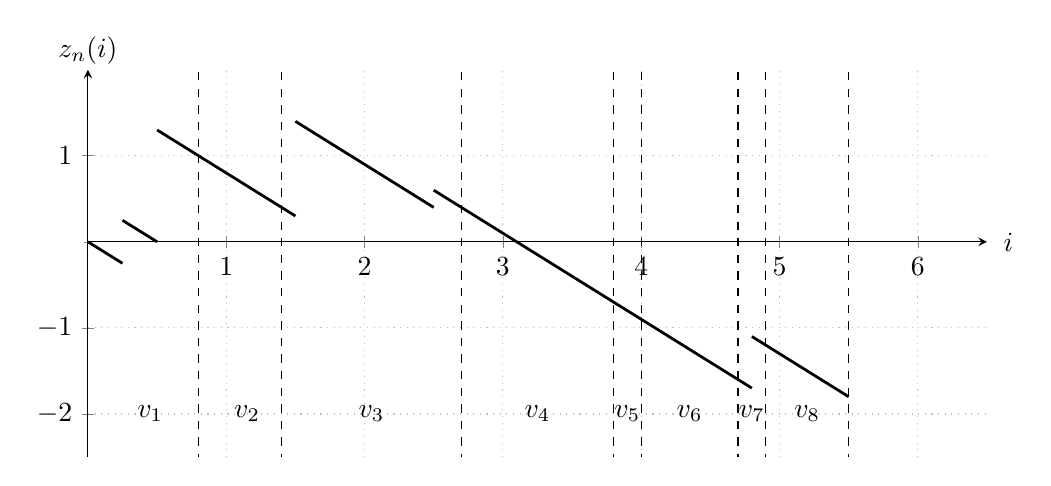
\begin{tikzpicture}

\begin{axis}[
axis x line=bottom,
axis y line=left,
grid = minor,
minor grid style={dotted},
xmin=0,
axis lines = middle,
xmax=6.5,
ymax = 2,
ymin  = -2.5,
xlabel={$i$},
x label style = {at={(axis description cs:1.04,0.555)},anchor=east},
ylabel={$z_n(i)$},
y label style = {at={(axis description cs:0,1.11)},anchor=north},
xtick={1,...,6},
minor xtick = {1,...,6},
ytick={-2,...,1},
minor ytick={-2,...,1},
width = 13cm,
height = 6.5cm
]


% BF WALK LINE
\addplot [line width=1.0pt]coordinates{(0,0) (0.25,-0.25)}; 
% JUMP 0.5
\addplot [line width=1.0pt]coordinates{(0.25,0.25) (0.5,0)}; 
% JUMP 1.3
\addplot [line width=1.0pt]coordinates{(0.5,1.3) (0.9,0.9)};

\addplot [line width=1.0pt]coordinates{(0.9,0.9) (1.5,0.3)}; 
% JUMP 1.1
\addplot [line width=1.0pt]coordinates{(1.5, 1.4) (2.5, 0.4)};
% JUMP 0.2
\addplot [line width=1.0pt]coordinates{(2.5, 0.6) (4.8,-1.7)};
% JUMP 0.6
\addplot [line width=1.0pt]coordinates{(4.8,-1.1) (5.5,-1.8)};

% VERTEX BORDERS
\addplot [dashed] coordinates {(0.8, -7) (0.8, 2)};
\addplot [dashed] coordinates {(1.4, -7) (1.4, 2)};
\addplot [dashed] coordinates {(2.7, -7) (2.7, 2)};
\addplot [dashed] coordinates {(3.8, -7) (3.8, 2)};
\addplot [dashed] coordinates {(4.0, -7) (4.0, 2)};
\addplot [dashed] coordinates {(4.7, -7) (4.7, 2)};
\addplot [dashed] coordinates {(4.9, -7) (4.9, 2)};
\addplot [dashed] coordinates {(5.5, -7) (5.5, 2)};

% VERETX LABELS
\node at (axis cs:0.45,-2) {$v_1$};
\node at (axis cs:1.15,-2) {$v_2$};
\node at (axis cs:2.05,-2) {$v_3$};
\node at (axis cs:3.25,-2) {$v_4$};
\node at (axis cs:3.9,-2) {$v_5$};
\node at (axis cs:4.35,-2) {$v_6$};
\node at (axis cs:4.8,-2) {$v_7$};
\node at (axis cs:5.2,-2) {$v_8$};

\end{axis}

\end{tikzpicture} }
	
	\caption{Continuous breadth-first walk components of the nonuniform random graph. Dashed lines indicate the end of vertices.}
	\label{F: nonu bf-walk}
\end{figure} 

Figure~\ref{F: nonu bf-walk} shows this construction for some sample components. 
We may think of the vertices $v_1, v_2, \dots$ occupying consecutive intervals on the time axis,
each the length of the interval for each vertex equal to its size.
During this time interval we search for children of the current vertex 
and each "birth" results in a jump of height equal to the size of the new vertex.

For the birth time $\beta(j)$ of $v_j$ as child of a vertex $v_i$ we have
\begin{equation}
	\beta(j) = \tau_{i-1} + \xi_{v_i, v_j}.
\end{equation}
For a vertex which is the root of its component, the birth time is simultaneously the start of its time interval:
\begin{equation}
	\beta(j) = \tau_{j-1}.
\end{equation}


%%%%%%%%%%%%%%%%%%%%%%%%%%%%%%%%%%%%%%%%%%%%%%%%%%%%%%%%%%%%%%%%%%%%%%%%%%%%%%%%
% THEOREM Z -> Wt nonuniform graph
%%%%%%%%%%%%%%%%%%%%%%%%%%%%%%%%%%%%%%%%%%%%%%%%%%%%%%%%%%%%%%%%%%%%%%%%%%%%%%%%
There now exists a direct equivalent to Theorem~\ref{T: Z -> W} for this nonuniform graph model and its breadth-first walk.

\begin{theorem} \label{T: Z -> W nonu}
	Let $\bfwn(s), 0 \leq s \leq \sum_{v} x^{(n)}_v$ be the breadth-first walk on $\Wrg(\xn, \qn)$.
	Define the rescaled breadth-first walk
	\begin{equation}
		\rbfwn(s) = \sqrt{\frac{\sign_2}{\sign_3}} \bfwn(s).
	\end{equation}
	Then
	\begin{equation}
		\rbfwn \rightarrow_d \Wt.
	\end{equation}	
\end{theorem}

For a complete proof of both theorems we refer to \cite[p.828ff.]{Aldous.1997}.
